% !TEX TS-program = pdftex
% !TEX encoding = UTF-8
% !BIB program = biber

\documentclass[12pt,a4paper]{report}

\usepackage{graphicx} % \includegraphics [k=v] interface za uključivanje grafike (slika, PDFa, ...)
\usepackage{bookmark} % generira ToC za PDF

% Podrška za hrvatski
\usepackage[croatian]{babel}
\usepackage{csquotes}

% Margine
\usepackage[left=3.5cm,top=1.5cm,right=3cm,bottom=4cm]{geometry}

% Simboli i naredbe za matematiku
\usepackage{amsmath, amsthm, amssymb}
\usepackage{mathtools}

% Poveznice
\usepackage{cleveref}
\usepackage{hyperref}

% Blokovi s kodom
\usepackage{minted}
\usemintedstyle{sas}

% Literatura
\usepackage[sorting=none,backend=biber,style=numeric]{biblatex}
\addbibresource{ref.bib}

% Fonts:
\usepackage[T1]{fontenc} % Allows specifying fonts
\usepackage{helvet} % Helvetica; phv
\usepackage{palatino} % Palatino; ppl

\gdef \title{Seminarski rad}
\gdef \class{Matematika 3}
\gdef \author{Tin Švagelj}
\gdef \uniprogram{Jednopredmetna Informatika}
\gdef \university{
Fakultet Informatike i Digitalnih Tehnologija\\
Rijeka
}
\gdef \semguide{dr.sc. Marija Maksimović}
\gdef \author{Tin Švagelj}
\gdef \date{\today}

\graphicspath{{./figures/}}

% Custom commands and redefinitions
\newcommand{\UseFont}[1]{\fontfamily{#1}\selectfont}

\usepackage{titlesec}
\titleformat{\chapter}[display]
{\normalfont\Large\bfseries}{\chaptertitlename\ \thechapter}{20pt}{\Large}

% \usepackage{fancyhdr}
% \pagestyle{fancy}
% \fancyhead{}
% \renewcommand\headrulewidth{0.1pt}
% \fancyhead[L]{\footnotesize \leftmark}
% \fancyhead[R]{\footnotesize \thepage}
% \renewcommand\headrulewidth{0pt}
% \fancyfoot[R]{\small Fakultet Informatike i\\Digitalnih Tehnologija}
% \renewcommand\footrulewidth{0.1pt}
% \fancyfoot[C]{2022 - 2023}
% \fancyfoot[L]{\small \title}

\begin{document}

\thispagestyle{empty}

\begin{titlepage}
	\begin{center}
		\vspace*{\stretch{0.25}}
		{\UseFont{phv} \Large \bf \title \par}
		{\large \em \UseFont{pzc} za kolegij \UseFont{phv} \class}\\ [.15\baselineskip] \par

		\vspace*{\stretch{0.3}}

		voditeljica kolegija:\\
		{\bf \semguide},\\
		\vspace*{10pt}
		student:\\
		{\bf \author}\\
		\UseFont{ppl} {\bfseries \uniprogram}

		\vspace*{\stretch{0.25}}
		
		\footnotesize{\bf \university} \par
		\bf{\date}
	\end{center}
\end{titlepage}

\pagenumbering{roman}

\tableofcontents
\newpage

\setcounter{page}{1}
\pagenumbering{arabic}

\chapter{Uvod}

Potrebno je odrediti ekstreme i nacrtati funkciju:
\begin{equation}
    \tag{\hspace{0pt}{$f$}\hspace{0pt}}
    \label{f_def}
    f(x, y) = 2x^3 + 2y^3 - 36xy + 430
\end{equation}

Bitno je odrediti domenu funkcije na početku kako bismo uspješno i smisleno odredili ekstreme funkcije jer mogu postojati samo unutar njene domene.\bigskip\par

Kako bismo mogli odrediti ekstreme funkcije, potrebno je odrediti nulte točke gradijenta ($\nabla$) funkcije\cite{ccalc}:
\begin{equation}
    \tag{{$\nabla f$}}
    \label{del_f}
    \nabla f(\mathbf{x}, \mathbf{y}) = \begin{bmatrix}
        \frac{\partial f}{\partial x} \\
        \frac{\partial f}{\partial y}
    \end{bmatrix}\textnormal{,}
\end{equation}

rješavajući sustav jednadžbi:
\begin{equation}
    \label{del_f_sys}
    \begin{cases}
        \frac{\partial f}{\partial x} = 0 \\
        \frac{\partial f}{\partial y} = 0 \textnormal{,}
    \end{cases}
\end{equation}

gdje su rješenje nulte točke funkcije gradijenta ($\nabla f(\mathbf{x}, \mathbf{y}) = 0$), tj. ekstremi funkcije \eqref{f_def}.\bigskip\par

Za određivanje parcijalne derivacije prvog reda funkcije koristimo pravila deriviranja \cite{kolegij}:

\begin{align}
    (c)' &= 0 \label{rule_const} \\
    (x^a)' &= ax^{a-1} \label{rule_exp} \\
    (f + g)' &= f' + g' \label{rule_sum}
\end{align}

\vspace*{20pt}

Crtanje će biti izvedeno koristeći \verb|NumPy| i \verb|Matplotlib| biblioteke u Python programskom jeziku.\par

\newpage

\chapter{Razrada}

S obzirom da je zadana funkcija \eqref{f_def} racionalna, važeća je za svaki $x \in \mathbb{R}$ i $y \in \mathbb{R}$ \cite[vidi][stranica 119]{kolegij}.
Dakle domena funkcije je skup svih realnih brojeva:
$$
    D(f) = \mathbb{R} \times \mathbb{R} = \mathbb{R}^2
$$

\section{Parcijalne derivacije prvog reda}

Kako bismo odredili gradijent funkcije \eqref{f_def}, trebamo prvo odrediti parcijalne derivacije te funkcije po $x$ i $y$, pri čemu se služimo pravilima \eqref{rule_const}, \eqref{rule_exp} i \eqref{rule_sum}:

\begin{align*}
    \frac{\partial f}{\partial x} & = \frac{\partial}{\partial x} (2x^3 + 2y^3 - 36xy + 430) \\
    & = \frac{\partial}{\partial x} 2x^3 + \frac{\partial}{\partial x}2y^3 - \frac{\partial}{\partial x}36xy + \frac{\partial}{\partial x}430 \\
    & = 6x^2 + 0 - 36y + 0 \\
    & = 6x^2 - 36y \\
    \\
    \frac{\partial f}{\partial y} & = \frac{\partial}{\partial y} (2x^3 + 2y^3 - 36xy + 430) \\
    & = \frac{\partial}{\partial y} 2x^3 + \frac{\partial}{\partial y}2y^3 - \frac{\partial}{\partial y}36xy + \frac{\partial}{\partial y}430 \\
    & = 0 + 6y^2 - 36x + 0\\
    & = 6y^2 - 36x \textnormal{.}
\end{align*}

S obzirom da je domena zadane funkcije \eqref{f_def} skup svih realnih brojeva, ne trebamo isključiti rješenja iz dobivenih izraza.

\newpage
\section{Crtanje grafa u Pythonu}

Za crtanje, kao što je već navedeno u uvodu, koristimo \verb|NumPy| i \verb|Matplotlib|.

\verb|NumPy|eva dokumentacija\cite{numpy_doc} i \verb|Matplotlib|ova specifikacija sučelja za programiranje aplikacija (engl. API Specification) \cite{mpl_api}, te upute za korištenje \cite{mpl_ug}, koji su dostupni putem interneta.

\verb|NumPy| omogućava podršku za rad s velikim, višedimenzionalnim poljima i matricama, zajedno sa širokim spektrom visoko-razinskih matematičkih funkcija.\par

Za početak rada je potrebno instalirati \verb|NumPy| i \verb|Matplotlib| pokretanjem \verb|pip install| naredbe u terminalu ili naredbenom retku:
\begin{minted}{shell}
    pip install --user numpy matplotlib
\end{minted}

Na početku svakog programa moramo uključiti potrebne module sa sljedećim kodom\cite[][naslov 5.4.2. Submodules]{py_lang_ref}:
\begin{minted}{python}
import numpy
import matplotlib.pyplot as plt
from mpl_toolkits.mplot3d import Axes3D
\end{minted}
, izvođenjem tih linija koda možemo pristupiti vanjskom koda u našim programima.

\subsection{NumPy}

Stvaramo jednodimenzionalne nizove (polja) od $100$ uniformno razmaknutih vrijednosti između $-10$ i $10$:
\begin{minted}{python}
x = np.linspace(-10, 10, 100)
y = np.linspace(-10, 10, 100)
\end{minted}
S obzirom da su ekstremi funkcije (rješenja) dobiveni od parametara koji se nalaze u intervalu $[-10, 10]$, uneseni argumenti funkcije će biti zadovoljavajući.\par
Nakon izvršavanja tog koda imamo \verb|x| i \verb|y| nizove sa 100 elemenata nalik na:
$$
    x = y = [-10,\space-9.8,\space-9.6,\dots,\space9.8,\space10]
$$

Zatim od ta dva jednodimenzionalna niza stvaramo dvodimenzionalni niz vrijednosti:
\begin{minted}{python}
X, Y = np.meshgrid(x, y)
\end{minted}
U našem slučaju se radi o $100\times100$ nizevima nalik na:
\begin{align*}
    X = Y^T = [&[-10,\space-9.8,\dots,\space9.8,\space10],\\
    &[-10,\space-9.8,\dots,\space9.8,\space10],\\
    &\hspace*{0.15\linewidth}\vdots\\
    &[-10,\space-9.8,\dots,\space9.8,\space10]]
\end{align*}

\newpage
\verb|NumPy| nam dozvoljava simboličko izražavanje funkcija,
pa za računanje \verb|Z| vrijednosti grafa, tj. rezultata funkcije \eqref{f_def} koji su nam
potrebni za crtanje grafa, možemo koristiti:
\begin{minted}{python}
Z = 2*X**3 + 2*Y**3 - 36*X*Y + 430
\end{minted}
, što će generirati novi dvodimenzionalni niz (dimenzija $100\times100$) s vrijednostima
funkcije \nameref{f_def} za sve uvrštene kombinacije $x$ i $y$ vrijednosti.\par
To je jedina linija koda koju moramo mjenjati za crtanje različitih grafova u ovom slučaju.\par
\verb|NumPy| u pozadini računa sve vrijednosti rezultirajućeg dvodimenzionalnog niza za sve odgovarajuće
parove\footnote{Parovi u rezultatu su usklađeni na osnovu stupca i retka} \verb|X| i \verb|Y| vrijednosti,
tj. za sve kombinacije \verb|x| i \verb|y| vrijednosti.

Time dobivamo dvodimenzionalni niz svih vrijednosti koje funkcija može poprimiti za sve kombinacije $x$ i $y$ u intervalima $[-10, 10]$:
$$
{{f(x,y) \mid x \in [-10, 10]} \mid y \in [-10, 10]}
$$

Razlog zašto možemo na tako prirodan način izraziti operacije nad multidimenzionalnim nizovima pomoću \verb|NumPy|a je zato što su
\verb|X| i \verb|Y| apstraktne reprezentacije nizeva za koje su definirani\footnote{Definirani kao preoptrećenja operatora u Pythonu} svi matematički operatori koje Python podržava za normalne brojeve.\par
Tako da nam \verb|X**3| prvo daje novi niz gdje je svaki element/broj iz niza \verb|X| eksponenciran brojem $3$.
Zatim je izraz \verb|2*X**3| evaluiran i zbog množenja rezultata sa $2$, \verb|NumPy| množi sve elemente niza sa $2$.
Na kraju vrši binarne operacije nad samim nizovima gdje dobivamo rješenja polinoma za cijeli izraz, te će taj rezultatski niz biti pohranjen u \verb|Z|.

Sada kada imamo sve vrijednosti koje funkcija poprima, možemo koristiti \verb|Matplotlib| za crtanje grafa. Za početak stvaramo 
\begin{minted}{python}
Z = 2*X**3 + 2*Y**3 - 36*X*Y + 430
\end{minted}

\newpage
\subsection{Matplotlib}

\verb|Matplotlib| pruža funkcije za crtanje širokog raspona statičkih, animiranih i interaktivnih vizualizacija.
Može se koristiti za stvaranje dijagrama stupčastih grafova, linijskih grafova, grafova raspršenja, pogrešnih traka,
histograma, dijagrama kružnica, dijagrama kutije i mnogih drugih vrsta vizualizacija.

Figura (engl. Figure) je u Matplotlib biblioteci cijelokupni prostor za crtanje koji može sadržavati jedan ili više grafova.
U napisanom kodu stvaramo novu figuru za crtanje te ju pohranjujemo u \verb|fig| varijablu:
\begin{minted}{python}
    fig = plt.figure()
\end{minted}

Stvaramo 3D podgraf unutar figure i pohranjujemo ga u \verb|ax| varijablu:

\begin{minted}{python}
    ax = fig.add_subplot(111, projection='3d')
\end{minted} 

Prvi argument (\verb|111|) određuje poziciju podgrafa unutar figure:
\begin{itemize}
    \item prvi broj određuje broj redaka,
    \item drugi broj stupaca,
    \item a treći broj indeks podgrafa.
\end{itemize}
U ovom slučaju, \verb|111| stvara jedan podgraf koji se proteže cijelom figurom. Ovaj argument nije obavezan jer smo koristili zadanu vrijednost, no naveden je u svrhu boljeg objašnjavanja figura.

Argument (\verb|projection|) specificira projekciju grafa, s obzirom da se radi o 3D grafu koristimo vrijednost \verb|'3d'|.
Potrebno je navesti projekciju jer je zadana vrijednost \verb|'rectilinear'| koja je zapravo ortogonalna projekcija usmjerena u ravninu s rješenjima $z = 0$ i koristi se za crtanje dvodimenzionalnih grafova.
Argumentom \verb|'3d'| navodimo da očekujemo ortogonalnu projekciju trodimenzionalnog grafa, koja gleda u smjeru:
$$
    \vec{v} = (\text{\it azimut}, \text{\it elevacija}) = (-60^{\circ}, 30^{\circ})
$$

U slučaju da želimo izmjeniti kut projekcije, to možemo postignuti korištenjem \verb|Axes3D.view_init()| funkcije:
\begin{minted}{python}
    ax.view_init(azim=azimut, elev=elevacija)
\end{minted}

Kako bismo nakon podešavanja grafa \verb|ax| ga konstruirali i nacrtali, potrebno je koristiti \verb|Axes3D.plot_surface(X, Y, Z)| funkciju za crtanje ravnina:
\begin{minted}{python}
    ax.plot_surface(X, Y, Z)
\end{minted}

Funkcije \verb|Axes3D.set_xlabel("x")|, \verb|Axes3D.set_ylabel("y")| i\\\verb|Axes3D.set_zlabel("z")| nam dozvoljavaju imenovanje $x$, $y$ i $z$ osi, sukladno redoslijedu:
\begin{minted}{python}
    ax.set_xlabel('x')
    ax.set_ylabel('y')
    ax.set_zlabel('$f(x,y)$')
\end{minted}

Korištenjem \verb|pyplot.savefig("putanja/do/datoteke.png")| možemo spremiti slike grafa u datotečnom sustavu:
\begin{minted}{python}
    plt.savefig("figures/graf_f.png")
\end{minted}

\newpage

\subsection{Grafovi funkcija}

Pokretanjem napisanog koda dobivamo graf:
\begin{figure}[H]
    \centering
    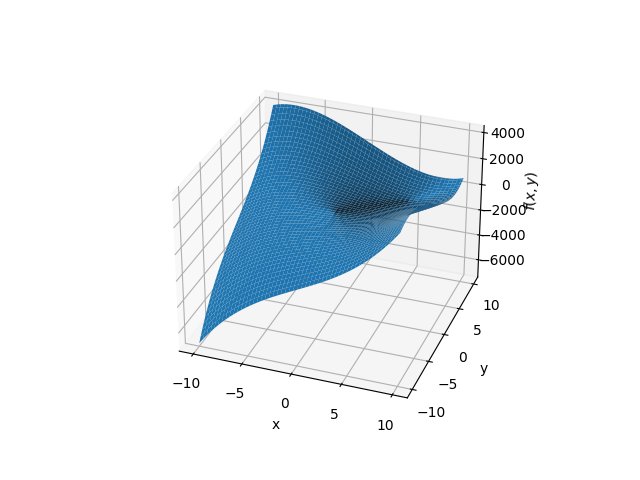
\includegraphics[width=400pt]{figures/graf_f.png}
    \caption{Graf zadane funkcije \eqref{f_def}}
\end{figure}

Promjenom vrijednosti \verb|Z|, parametara \verb|ax|, i ciljane datoteke možemo nacrtati i grafove parcijalnih derivacija funkcije po $x$ i $y$:
\begin{figure}[H]
    \begin{subfigure}{0.5\linewidth}
        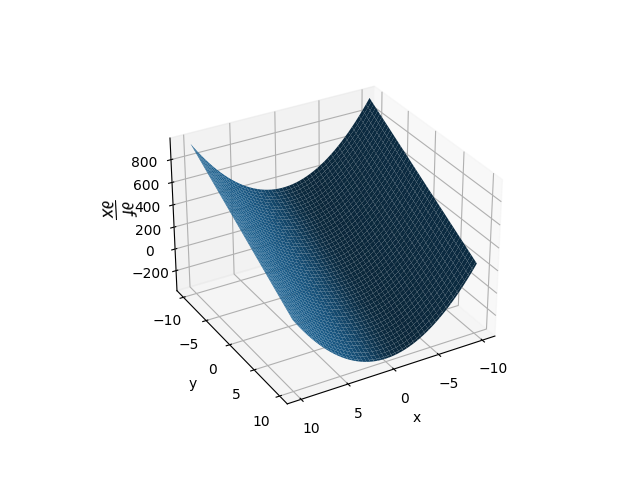
\includegraphics[width=200pt]{figures/graf_fdx.png}
        \caption{Parcijalna derivacije funkcije po $x$}
    \end{subfigure}%
    \begin{subfigure}{0.5\linewidth}
        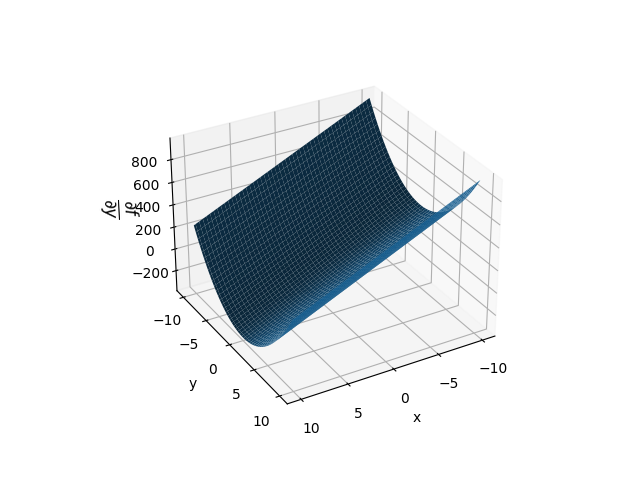
\includegraphics[width=200pt]{figures/graf_fdy.png}
        \caption{Parcijalna derivacije funkcije po $y$}
    \end{subfigure}
    \caption{Grafovi parcijalnih derivacija}
\end{figure}

\newpage
\section{Gradijent funkcije}

Određujemo gradijent \eqref{del_f} funkcije \eqref{f_def} uz dobivene parcijalne derivacije:

\begin{equation}
    \nabla f(\mathbf{x}, \mathbf{y}) = \begin{bmatrix}
        6x^2 - 36y \\
        6y^2 - 36x
    \end{bmatrix}\textnormal{,}
\end{equation}

\section{Ekstremi}

Gradijent \eqref{del_f} izjednačujemo s nulom kako bi mu odredili nulte točke tj. ekstreme funkcije.
To možemo izraziti kao sustav \eqref{del_f_sys}:

$$
\begin{cases}
    6x^2 - 36y = 0 \\
    6y^2 - 36x = 0 \textnormal{.}
\end{cases}
$$

Izrazimo $y$ iz prve jednadžbe sustava,
\begin{align*}
    6x^2 - 36y &= 0 \\
    36y &= 6x^2 \\
    y &= \frac{6x^2}{36} = \frac{x^2}{6}
\end{align*}

te $y$ substituiramo u drugu jednadžbu kako bismo dobili jednadžbu za $x$eve nultih točaka gradijenta:
\begin{align}
    6(\frac{x^2}{6})^2 - 36x &= 0 \nonumber \\
    \frac{x^4}{6} - 36x &= 0 \nonumber \\
    x^4 - 6^3x &= 0 \label{del_fx_zeros}
\end{align}

Jedno rješenje ($x_1$) uočavamo nakon izlučivanja $x$a iz izraza:
\begin{align*}
    x(x^3 - 6^3) &= 0 \\
    x_1 &= 0 \textnormal{.}
\end{align*}

Zaključujemo da je jedno rješenje $x_1 = 0$ jer ako je $x$ jednak nuli, onda će jednadžba za $x$ nultih točaka gradijenta \eqref{del_fx_zeros} vrijediti. \par

Drugi član umnoška nam daje drugo rješenje:
\begin{align*}
    x^3 - 6^3 &= 0 \\
    x^3 &= 6^3 \\
    x &= \sqrt[3]{6^3} = 6 \textnormal{,}
\end{align*}

Time dobivamo 2 rješenja sustava za $x$:
\begin{gather*}
    x_1 = 0 \qquad x_2 = 6
\end{gather*}

Za $x_1 = 0$, $y_1$ će biti $0$. $y_2$ računamo uvrštavajući dobivene vrijednosti $x_2$ u jednu od parcijalnih derivacija:

\begin{align*}
    6x^2 - 36y &= 0\\
    6^3 - 36y &= 0\\
    36y &= 6^3\\
    y &= 6
\end{align*}

Time utvrđujemo da su realni ekstremi funkcije \eqref{f_def}:

\begin{center}
\begin{tabular}{c | c}
    $x$ & $y$ \\
    \hline
    $0$ & $0$ \\
    $6$ & $6$ \\
\end{tabular}
\end{center}

\newpage
\chapter{Zaključak}

Korištenjem \verb|NumPy| i \verb|Matplotlib| biblioteka u Pythonu, pomoću sljedećeg koda možemo dobiti 3D prikaz cijele multivarijatne funkcije:

\inputminted{python}{./code/graf_fje.py}

\begin{figure}
    \centering
    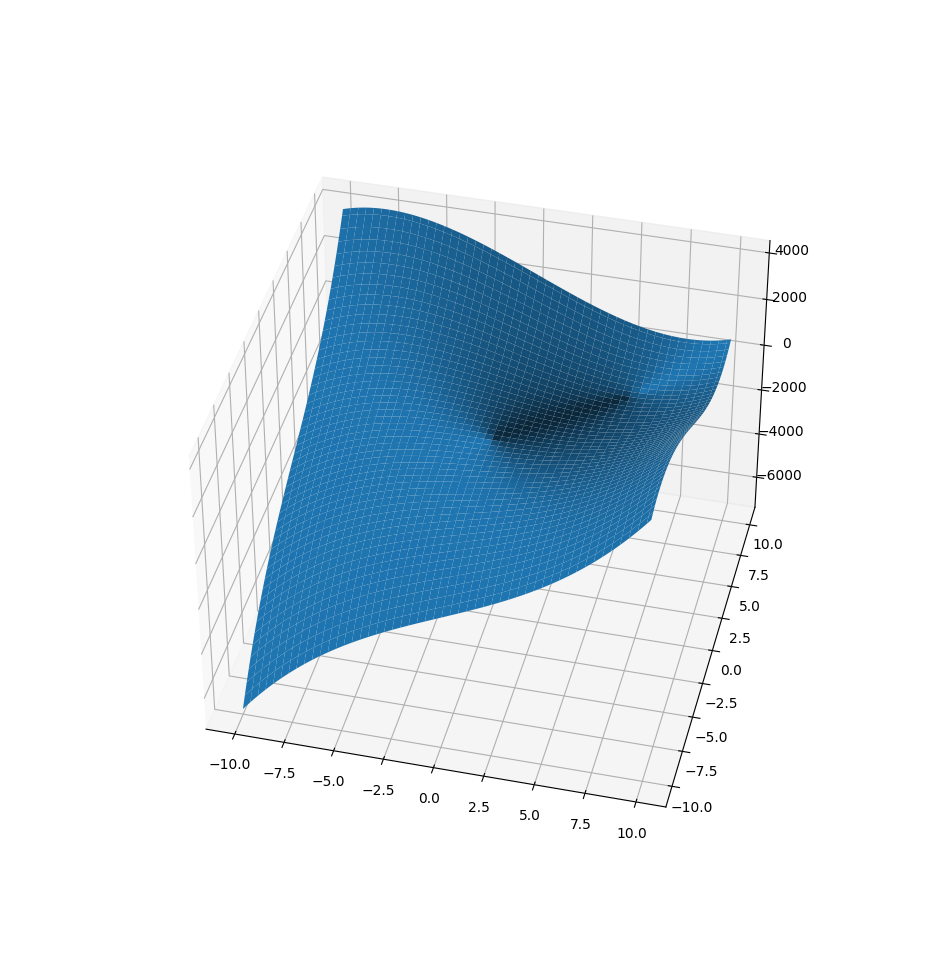
\includegraphics[width=0.8\textwidth]{graf_fje}
    \caption{Graf zadane funkcije \eqref{f_def}}
\end{figure}

Na grafu vidimo da dobivene točke jesu ekstremi funkcije. \par
Za algebarsko određivanje o kakvim se ekstremima radi bi trebali odrediti Hessovu matricu i parcijalne derivacije višeg reda \cite[][poglavlje 6.3]{ccalc}, no to nije traženo u sklopu ovog zadatka.

\newpage


\pagenumbering{roman}
\setcounter{page}{2}

\printbibliography[heading=bibintoc,title=Literatura]

\end{document}
